% Spectral analysis of the MRIxFields 2026 data -- short deck.
% Part 1 figures are the stored outputs of Dieleman's notebook (extracted to
% reports/spectral/dieleman/); Part 2 numbers come from reports/spectral/alpha_summary.csv
% (retrospective split, n = 30 per cell).
% Audience knows MRI, DL/ML and statistics but not spectral-analysis vocabulary: every term is
% expanded on the slide where it first appears. Avoid "decade" and "octave" entirely.
% Build: pdflatex -interaction=nonstopmode spectral_slides.tex   (twice, for the frame counter)
\documentclass[aspectratio=169,11pt]{beamer}

\usetheme{default}
\usepackage{lmodern}
\usepackage[T1]{fontenc}
\usepackage{amsmath}
\usepackage{booktabs}
\usepackage{graphicx}

\setbeamertemplate{navigation symbols}{}
\setbeamertemplate{footline}[frame number]
\setbeamercolor{frametitle}{fg=black}
\setbeamercolor{structure}{fg=black!70}
\setbeamerfont{frametitle}{size=\large,series=\bfseries}
\setbeamertemplate{itemize item}{\textbf{--}}

\definecolor{accent}{HTML}{1F4E79}
\definecolor{warn}{HTML}{9C2B2B}
% Must match SIGNAL_COLOUR / NOISE_COLOUR / SUM_COLOUR in scripts/make_noise_schematic.py.
\definecolor{sigred}{HTML}{CF2E2E}
\definecolor{noiseblue}{HTML}{2B3FD4}
\definecolor{sumgreen}{HTML}{2F6B3A}
\newcommand{\hl}[1]{\textcolor{accent}{\textbf{#1}}}
\newcommand{\bad}[1]{\textcolor{warn}{\textbf{#1}}}

% Small part label above the frame title; grey gloss line for terminology; figure source line.
\newcommand{\parttag}[1]{{\scriptsize\textcolor{gray}{#1}}\par\vspace{0.3em}}
\newcommand{\gloss}[1]{{\footnotesize\textcolor{black!65}{#1}}\par}
\newcommand{\srcline}[1]{\vfill{\scriptsize\textcolor{gray}{#1}}}

\newenvironment{airy}
  {\begin{itemize}\setlength{\itemsep}{0.9em}}
  {\end{itemize}}

\begin{document}

% ============================================================ PART 1 ========
\begin{frame}{Image Spectra}
  \parttag{PART 1 \quad Decompose images into frequency components}

  \centering
  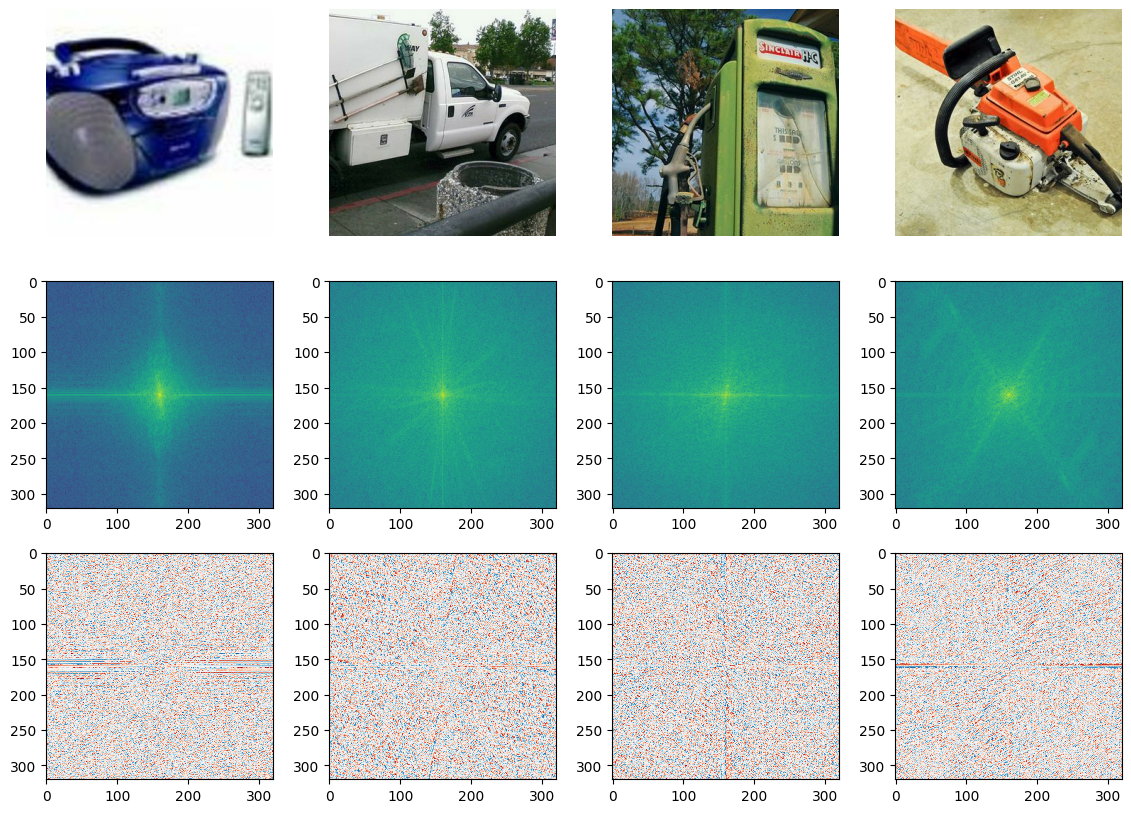
\includegraphics[height=0.56\textheight]{spectral/dieleman/cell16.png}

  \vspace{0.4em}
  \raggedright
  \gloss{Fourier Transform of each photo. \\
  \textbf{Middle row} -- Magnitude spectrum \\
  \textbf{Bottom row} -- Phase spectrum.
  }

  \srcline{Figures throughout Part 1: Dieleman, \emph{Diffusion is spectral autoregression} (2024).}
\end{frame}

% ---------------------------------------------------------------------------
\begin{frame}{Collapse to one curve per image}
  \parttag{PART 1 \quad A formal way to reason on different scales of features in images}

  \centering
  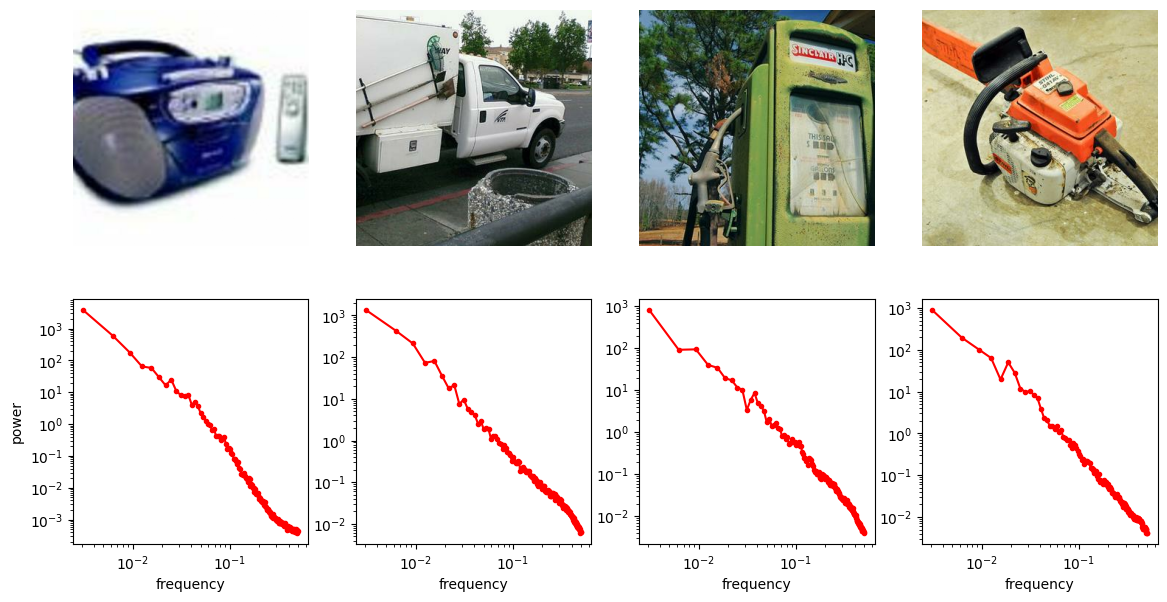
\includegraphics[height=0.56\textheight]{spectral/dieleman/cell21.png}

  \vspace{0.5em}
  \raggedright
  \gloss{Average the magnitude spectrum over all directions observe the \emph{power--frequency} plot at log-log scale. \\
  Averaging algorithm is \hl{RAPSD} -- \emph{radially averaged power spectral density}.
  }
\end{frame}

% ---------------------------------------------------------------------------
\begin{frame}{Average over a dataset}
  \parttag{PART 1 \quad Natural image tends to approximately follow \textbf{power law}}

  \begin{columns}[c,onlytextwidth]
  \begin{column}{0.4\textwidth}
    \[ \textbf{$P (f)$} \;\propto\; f^{-\alpha} \]

    \small
    \begin{itemize}\setlength{\itemsep}{0.4em}
      \item \hl{$\alpha$ is the slope} of the dotted line -- higher $\alpha$ suggests a faster decay in high frequency.
      \item Natural Images: \hl{$\alpha \approx 2$}\,\textsuperscript{1,2,3}. About every order of magnitude contributes equally.
    \end{itemize}
  \end{column}

  \begin{column}{0.58\textwidth}
    \centering
    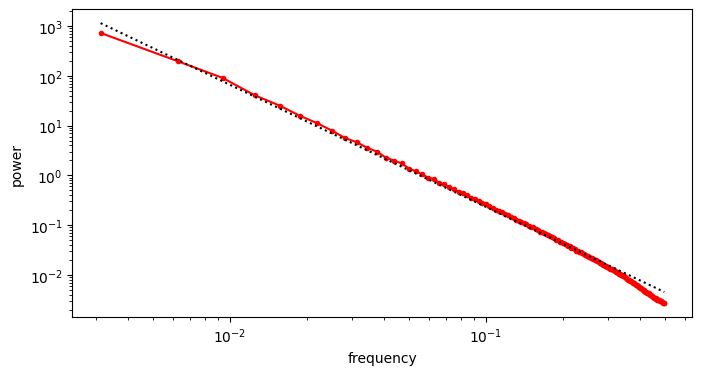
\includegraphics[width=0.88\linewidth]{spectral/dieleman/cell28.png}
  \end{column}
  \end{columns}

  \srcline{Dotted line: least-squares fit. A straight line on log--log axes which \emph{is} a power law.}

  \vspace{0.25em}
  {\tiny\textcolor{gray}{%
  \textsuperscript{1}van der Schaaf \& van Hateren, ``Modelling the Power Spectra of Natural Images:
  Statistics and Information'', \emph{Vision Research}, 1996. \\
  \textsuperscript{2}Torralba \& Oliva, ``Statistics of natural image categories'',
  \emph{Network: Computation in Neural Systems}, 2003. \\
  \textsuperscript{3}Hyv\"arinen, Hurri \& Hoyer, \emph{Natural Image Statistics: A Probabilistic
  Approach to Early Computational Vision}, 2009.}\par}
\end{frame}

% ---------------------------------------------------------------------------
\begin{frame}{Adding noise destroys fine detail first}
  \parttag{PART 1 \quad What is already known about natural photographs}

  \centering
  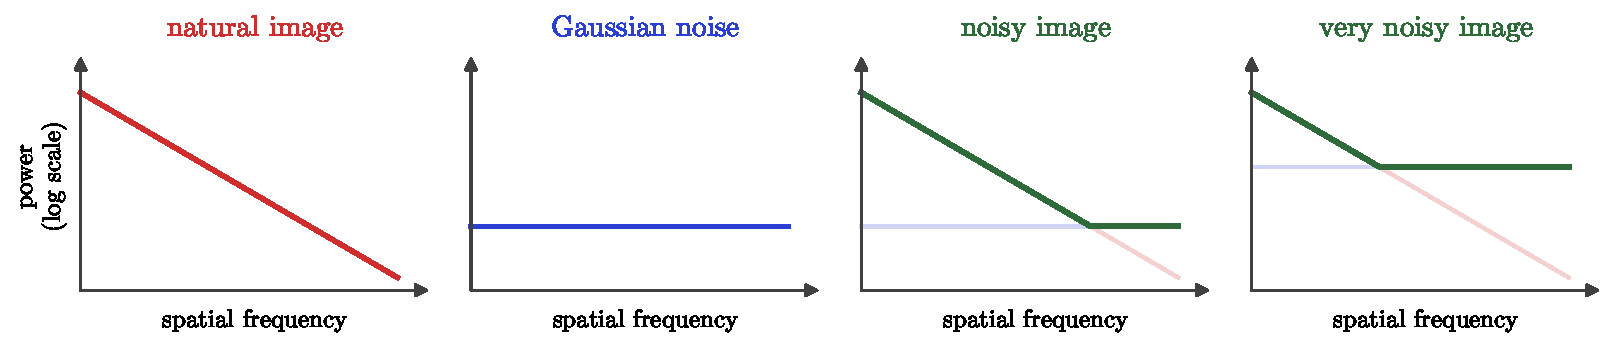
\includegraphics[width=\textwidth]{spectral/fig_noise_schematic.pdf}

  \vspace{0.8em}
  \begin{columns}[c,onlytextwidth]
  \begin{column}{0.58\textwidth}
    \raggedright
    \gloss{\textcolor{sigred}{\textbf{red}}: Image,
           \textcolor{noiseblue}{\textbf{blue}}: Gaussian noise,
           \textcolor{sumgreen}{\textbf{green}}: Noisy Image}

    \vspace{0.7em}
    \gloss{$\Rightarrow$ Denoising in reverse rebuilds images via \hl{coarse first, fine detail last}. \\ 
    The noise schedule of a diffusion model is kind of a \hl{detail schedule}, and $\alpha$ controls how fast it moves. \\
    }
    \gloss{$\Rightarrow$ Considering this, it can also suggest how well a diffusion model can learn to generate fine detail on a given dataset.}
  \end{column}
  \begin{column}{0.38\textwidth}
    \centering
    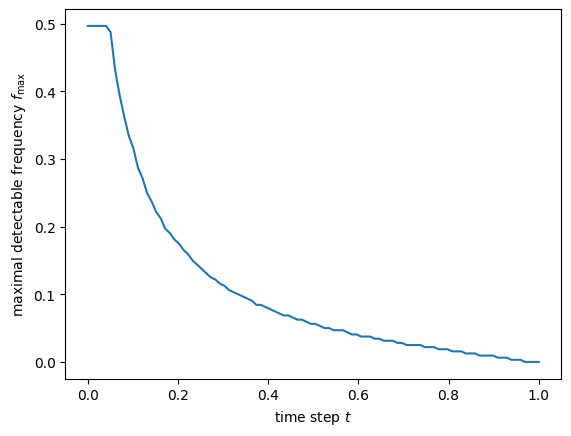
\includegraphics[width=0.78\linewidth]{spectral/dieleman/cell43.png}
  \end{column}
  \end{columns}

  \raggedright
  \srcline{Schematic redrawn after Dieleman (2024).}
\end{frame}

% ============================================================ PART 2 ========
\begin{frame}{Measuring on MRI data, steeper slopes}
  \parttag{PART 2 \quad MRIxFields \qquad {\itshape 30 volumes per cell; slope fitted between 0.02 and 0.2 cycles/pixel}}

  \centering
  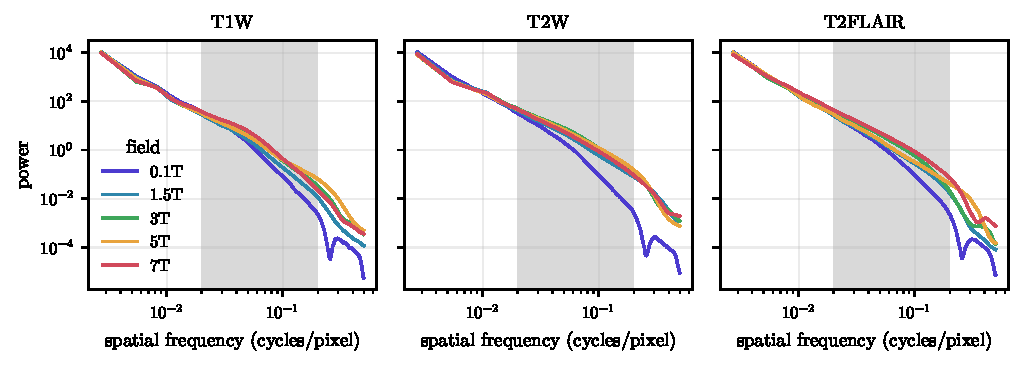
\includegraphics[width=0.82\textwidth]{spectral/fig_rapsd_by_field_retro.pdf}

  \vspace{0.5em}
  \begin{tabular}{lccccc|c}
    \toprule
    slope $\alpha$ & 0.1\,T & 1.5\,T & 3\,T & 5\,T & 7\,T & natural images \\
    \midrule
    mean over modalities & \bad{4.16} & 3.09 & 2.93 & 2.71 & 2.89 & \hl{$\approx 2$} \\
    \bottomrule
  \end{tabular}

  \vspace{0.4em}
  \raggedright
  \gloss{Steeper than natural images -- MRI is band-limited by acquisition and
  reconstruction. \\
  \bad{0.1\,T is the outlier} (low SNR forces averaging and heavy denoising). \\
  Low $\sigma$ above 1.5\,T meaning, protocol matters more than field strength: \hl{\textit{high base acquisition bias}}
  }
\end{frame}

% ---------------------------------------------------------------------------
\begin{frame}{Task 1 is two different problems}
  \parttag{PART 2 \quad MRIxFields}
  \vfill

  \begin{columns}[c,onlytextwidth]
  \begin{column}{0.5\textwidth}
    \centering\scriptsize
    \setlength{\tabcolsep}{4pt}

    fitted slope $\alpha$\par
    \vspace{0.2em}
    \begin{tabular}{lccccc}
      \toprule
       & 0.1\,T & 1.5\,T & 3\,T & 5\,T & 7\,T \\
      \midrule
      T1W     & \bad{4.32} & 3.47 & 3.14 & 2.80 & 3.31 \\
      T2W     & \bad{4.16} & 2.76 & 2.60 & 2.45 & 2.66 \\
      T2FLAIR & \bad{3.99} & 3.04 & 3.04 & 2.88 & 2.69 \\
      \bottomrule
    \end{tabular}

    \vspace{1.2em}
    same numbers minus the 7\,T target\par
    \vspace{0.2em}
    \begin{tabular}{lcccc}
      \toprule
       & 0.1\,T & 1.5\,T & 3\,T & 5\,T \\
      \midrule
      T1W     & \bad{$+1.01$} & $+0.16$ & $-0.17$ & $-0.51$ \\
      T2W     & \bad{$+1.50$} & $+0.10$ & $-0.06$ & $-0.21$ \\
      T2FLAIR & \bad{$+1.29$} & $+0.35$ & $+0.34$ & $+0.18$ \\
      \bottomrule
    \end{tabular}
  \end{column}

  \begin{column}{0.46\textwidth}
    \small
    \begin{airy}
      \item \bad{Positive $=$ input missing detail.} 0.1\,T holds only ${\sim}3\%$ of 7\,T's
            fine detail. It was never acquired, so it must be \emph{generated}.
      \item \hl{Negative $=$ input has too much.} 3\,T and 5\,T are already finer than 7\,T --
            the right map is a slight blur. Hence copying the input scores well.
      \item \bad{nRMSE cannot tell these apart:} the finest detail holds ${\sim}5\%$ of the variance
            the coarsest does.
    \end{airy}
  \end{column}
  \end{columns}
  \vfill
\end{frame}

% ---------------------------------------------------------------------------
\begin{frame}{What we change}
  \parttag{PART 2 \quad MRIxFields}

  \begin{columns}[T,onlytextwidth]
  \begin{column}{0.49\textwidth}
    \textbf{1. Generate only what is missing}

    \vspace{0.5em}
    {\small The input is already right at coarse scales, and that is where nearly all the variance is.

    \vspace{0.6em}
    So blur the input where it deviates from target curve, and let decoder produce
    \hl{missing high frequency detail}.

    \vspace{0.6em}
    Cascaded super-resolution with the split \emph{measured}?}
  \end{column}

  \begin{column}{0.49\textwidth}
    \textbf{2. Use the slope as a metric}

    \vspace{0.5em}
    {
      \small Fit the slope on the \emph{outputs of the model}, compare to the target's.

      \vspace{0.2em}
      \[ R(f) = \log S_{\hat x}(f) - \log S_x(f) \]
      \par\vspace{0.1em}
      \gloss{$S$: RAPSD function \quad $\hat x$: prediction}
      \vspace{0.1em}
      \gloss{$x$: target \quad $R$: log-ratio curve}

      \vspace{0.6em}
      A blurring model gives \hl{a steeper slope than the target} -- visible long before nRMSE moves.

      \vspace{0.6em}
      Cheap, fast and easy to implement.
    }
  \end{column}
  \end{columns}

  \srcline{Caveats: real curves bend slightly; in-plane only (no z-axis measurement); most cross field strengths have
  disjoint subjects.}
\end{frame}

\end{document}
